\documentclass[12pt]{article}
\usepackage{a4wide}
\usepackage{latexsym}
\usepackage{amssymb}
\usepackage{amsmath}
\usepackage{epic}
\usepackage{graphicx}
\newcommand{\tr}{\mbox{\sf true}}
\newcommand{\fa}{\mbox{\sf false}}
\newcommand{\bimp}{\leftrightarrow}


\begin{document}

\section*{Report for assignments for Automated Reasoning}

\begin{center}
\textbf{Authors}: \\
\begin{tabular}{rcl}
Dibran Dokter & s1047390 & {\tt dibran.dokter@ru.nl} \\
Sijmen van Bommel & s1038820 
\end{tabular}
\end{center}

\vspace{8mm}

\subsection*{Problem 1: Pallets}

Eight trucks have to deliver pallets of obscure building blocks to a magic factory. Every truck
has a capacity of 8000 kg and can carry at most eight pallets. In total, the following has to
be delivered: \\
\begin{itemize}
    \item Four pallets of nuzzles, each of weight 700 kg.
    \item A number of pallets of prittles, each of weight 400 kg.
    \item Eight pallets of skipples, each of weight 1000 kg.
    \item Ten pallets of crottles, each of weight 2500 kg.
    \item Twenty pallets of dupples, each of weight 200 kg.
\end{itemize}

\vspace{8mm}

Skipples need to be cooled; only three of the eight trucks have facility for cooling skipples. \\
Nuzzles are very valuable: to distribute the risk of loss no two pallets of nuzzles may be
in the same truck. \\
1. Investigate what is the maximum number of pallets of prittles that can be delivered,
and show how for that number all pallets may be divided over the eight trucks.\\
2. Do the same, with the extra information that prittles and crottles are an explosive
combination: they are not allowed to be put in the same truck.\\

\vspace{8mm}

\newpage

\subsubsection*{Solution:}

We start by defining a 2 dimensional array of integer values $trucks$ for the number of trucks ($ntrucks$) and the number of different pallets ($npallettypes$). \\
This leads to a $n \times k$ array of integers where n is the number of trucks and k is the number of pallet types. \\
 Where the integer value $ trucks_{i,j} $ is the number of pallets of type $j$ in truck $i$. \\

Besides this list we have a list for the weights for the different types of pallets, this list is used as a lookup table. \\
\[ weightlookup = [nuzzlesweight, prittlesweight, skipplesweight, crottlesweight, dupplesweight] \]
which for this specific case is:
\[ weightlookup = [700, 400, 1000, 2500, 200] \]
We define another list for the number of pallets that are required for the different types of pallets.\\
\[ itemtypes = [nuzzlesreq, prittlesreq, skipplesreq, crottelsreq, dupplesreq] \]
which for this specific instance is:
\[ itemtypes = [4, 0, 8, 10, 20] \] \\
Where the 0 for the number of prittles means we want to put as many as possible since there is no limit.\\

After this we can start defining the different constraints on the solution.\\

All the number of pallets on the trucks must be non-negative: \\
\[ nonnegative = \bigwedge_{i=1}^{ntrucks} \bigwedge_{j=1}^{itemtypes} (trucks_{i,j} \geq 0). \]

Constrain the weight of the pallets per truck. we do this by looking up the weight of the itemtype and multiplying it by the number of pallets of that type for every itemtype. Then we sum these for every truck and check if the total weight us under the maximum weight: \\
\[ weight = \bigwedge_{i=1}^{ntrucks} ( \sum_{j=1}^{itemtypes} (weighttable_j \cdot trucks_{i,j} ) \leq maxweight. \]

Constrain the capacities of the pallets per truck by summing the number of items per truck: \\
\[ capacities = \bigwedge_{i=1}^{ntrucks} \sum_{j=1}^{itemtypes} ( trucks_{i,j} ) \leq capacity \]

For each pallet type, require at least the given number of pallets, except for the prittles, example for nuzzles:
\[ nuzzles = \sum_{i=1}^{ntrucks} \left( trucks_{i,nuzzles} \right)  \geq nuzzlesrequired \]
This can be generalized as follows:
\[ items = \bigwedge_{j=1}^{itemtypes} \sum_{i=1}^{trucks} ( trucks_{i,j} ) \geq itemsrequired_j  \]

After defining these constraints the basic case without the cooling or distribution of nuzzles is satisfied.

Then we define the further constraints as follows. \\

\textbf{Skipples need to be cooled} \\
Only three of the eight trucks have facility for cooling skipples\\
We do this by taking all the non-cooled trucks and making sure there are 0 nuzzles in them:
\begin{align}
ncooledtrucks = 3 \\
cooledskipples = \bigwedge_{i=ncooledtrucks + 1}^{notcooledtrucks} (trucks[i][nuzzles] == 0)
 \end{align}

\textbf{Nuzzles are very valuable} \\
To distribute the risk of loss no two pallets of nuzzles may be in the same truck:

\[ valuablenuzzles = \bigwedge_{i=1}^{ntrucks} (trucks_{i,nuzzles} < 2) \]

Now we have all constraints, the total formula consists of the conjunction of all these constraints:
\[ nonnegative \wedge capacities \wedge items \wedge cooledskipples \wedge valuablenuzzles  \]

\subsubsection*{1.}

Investigate what is the maximum number of pallets of prittles that can be delivered,
and show how for that number all pallets may be divided over the eight trucks. \\

After defining these constraints we optimise for the number of prittles by using the z3 Optimizer, and we
define the following requirement:
\[ \bigwedge_{i=1}^{ntrucks} maximize(trucks_{i,prittles}) \]

Applying {\tt python trucks.py} yields the following result within half a second:
 
{\tt [0, 5, 1, 2, 0] }

{\tt [0, 4, 3, 1, 0] }

{\tt [0, 0, 4, 0, 4] }

{\tt [1, 0, 0, 2, 5] }

{\tt [1, 0, 0, 2, 5] }

{\tt [1, 5, 0, 1, 1] }

{\tt [0, 8, 0, 0, 0] }

{\tt [1, 0, 0, 2, 5] } \\

which contains:\\
$ 5 + 4 + 0 + 0 + 0 + 5 + 8 + 0  = 22 $ prittles

\subsubsection*{2.}

Do the same, with the extra information that prittles and crottles are an explosive
combination: they are not allowed to be put in the same truck.
We restrict the model that not both prittles and crottles can have a capacity of more than zero for each truck. :
\[ \bigwedge_{i=1}^{ntrucks} \neg (trucks_{i,prittles}>0 \wedge trucks_{i,crottles}>0) \]


Again applying {\tt python trucks.py} yields the following result within 4 seconds: \\

{\tt [0, 0, 2, 2, 4] }

{\tt [1, 0, 2, 2, 1] }

{\tt [0, 4, 4, 0, 0] }

{\tt [1, 0, 0, 2, 5] }

{\tt [0, 8, 0, 0, 0] }

{\tt [0, 8, 0, 0, 0] }

{\tt [1, 0, 0, 2, 5] }

{\tt [1, 0, 0, 2, 5] } \\

This solution has $ 4 + 8 + 8 = 20 $ prittles

\subsubsection*{Generalization}

Our solution can be generalized by giving a different number for $ntrucks$ and $npallettypes$ and defining a different lookup list for the weights and required number of pallets per type.

This way the problem can be generalized to fitting any number of items in any number of trucks according to some weight limit and required items.

The problem is scale-able by changing these values but this will negatively impact the performance for a big enough number of trucks and required pallets since it has to check a larger space for a solution.

\subsection*{Problem 2: Chip Design}

\subsubsection*{Problem}

Give a chip design containing two power components and ten regular components satisfying the following constraints:\\
\begin{itemize}
    \item Both the width and the height of the chip is 30.
    \item The power components have width 4 and height 3.
    \item The sizes of the ten regular components are 4 × 5, 4 × 6, 5 × 20, 6 × 9, 6 × 10, 6 × 11, 7 × 8, 7 × 12, 10 × 10, 10 × 20, respectively.
    \item All components may be turned $90^\circ$, but may not overlap.
    \item In order to get power, all regular components should directly be connected to a power component, that is, an edge of the component should have a part of length > 0 in common with an edge of the power component.
    \item Due to limits on heat production the power components should be not too close: their centres should differ at least 16 in either the x direction or the y direction (or both).
\end{itemize}

What if this last distance requirement of 16 is increased to 17? And what if it is increased to 18?

\subsubsection*{Solution}

First we define a data structure which will hold the different components of the chip. This is a 2 dimensional array with the different $components$ and their $attributes$.\\
A component has the following attributes: X position on the top-left corner of the chip, Y position on the top-left corner of the chip, the width of the component and the height of the component.\\

Besides this we have a list of components where every component has its corresponding width and height. So $components = [(4,3),(4,3),(4,5),...]$ for the power components and the regular components.\\
From this list of components we take the first 2 components to be the power components, so $powercomponents = [ components_0, components_1 ]$

After defining this data structure we define the following constraints:

The constraint that the X and Y values for the different components have to be within the $30 \times 30$ bounds of the size of the chip. We do this by checking the X and Y values for all the components and ensuring they are within the width and height of the chip:

\[ \begin{array}{c} \bigwedge_{c=1}^{components} chip_{c,X} \geq 0 \land chip_{c,Y} \geq 0  \\
\land chip_{c,X} + chip_{c,Width} \leq ChipWidth \land chip_{c,Y} + chip_{c,Height} \leq ChipHeight 
\end{array} \]
%# x and y at least 0 and not bigger than width and height (minus 1)
%in_bounds_c = [And(chip[comp][COMP_X] >= 0, chip[comp][COMP_Y] >= 0, chip[comp][COMP_X] + chip[comp][COMP_WIDTH]
%                   <= WIDTH, chip[comp][COMP_Y] + chip[comp][COMP_HEIGHT] <= HEIGHT) for comp in range(NO_COMPONENTS)]

The constraint that the components on the chip have to adhere to the sizes of the components from the components list.
The components on the chip can be rotated so they either have to match the standard orientation or the rotated orientation. We do this by checking that any component on the chip has the same width and height as either the normal orientation of a component in the components list or a rotated orientation of a component in the components list:

\[ \begin{array}{c} \bigwedge_{c=1}^{components} \left( chip_{c,Width} == components_{c,Width} \land chip_{c,Height} == components_{c,Height} \right) \\
\lor \left( chip_{c,Width} == components_{c,Height} \land chip_{c,Height} == components_{c,Width} \right)
\end{array} \]
%# chip of right size
%correct_size_c = [Or(And(chip[comp][COMP_WIDTH] == components[comp][0], chip[comp][COMP_HEIGHT] == components[comp][1]),
%                     And(chip[comp][COMP_WIDTH] == components[comp][1], chip[comp][COMP_HEIGHT] == components[comp][0])) for %comp in range(NO_COMPONENTS)]

The constraint that chips cannot overlap. We do this by taking 2 different components and ensuring they do not overlap, we do this for all components. We check if component do not overlap by checking if one component is either above, below, left or right from another component.

we define a lambda function:
\[ \begin{array}{c} Overlap_{c1,c2} = chip_{c2,X} \geq ( chip_{c1,X} + chip_{c1,Width} ) \lor chip_{c2,Y} \geq chip_{c1,Y} + chip_{c1,Height} \\
\lor (chip_{c2,X} + chip_{c2,Width}) \leq chip_{c1,X} \lor ( chip_{c2,Y} + chip_{c2,Height} ) \leq chip_{c1,Y}
\end{array} \]
for every two components:
\[ \bigwedge_{c1=1}^{components} \bigwedge_{c2=1}^{components} \left( c1 < c2 \land Overlap_{c1,c2}\right)  \]
%# chips cannot overlap, take 2 different components and ensure they do not overlap, do this for all components
%overlap_c = []
%for c1 in range(NO_COMPONENTS):
%    for c2 in range(NO_COMPONENTS):
%        if (c1 < c2):
%            overlap_c.append(Or(chip[c2][COMP_X] >= chip[c1][COMP_X] + chip[c1][COMP_WIDTH], chip[c2][COMP_Y] >= chip[c1][COMP_Y] + chip[c1][COMP_HEIGHT],
%                             chip[c2][COMP_X] + chip[c2][COMP_WIDTH] <= chip[c1][COMP_X], chip[c2][COMP_Y] + chip[c2][COMP_HEIGHT] <= chip[c1][COMP_Y]))

In order to get power, all regular components should directly be connected to a power component, that is, an edge of the component should have a part of length $> 0$ in common with an edge of the power component: \\
For this we take the components without the powercomponents and just the powercomponents and we define this constraint in 2 parts, first we check if the chip is connected above or below the power chip:\\

\[ \begin{array}{c} aboveOrBelow =\\ \bigwedge_{c=1}^{components} \bigwedge_{pc=1}^{powercomponents} chip_{c,X} < (chip_{pc,X} + chip_{pc,Width})  \land (chip_{c,X} + chip_{c,Width}) > chip_{pc,X} \\
\land (chip_{c,Y} + chip_{c,Height} == chip_{pc,Y} \lor chip_{c,Y} == chip_{pc,Y} + chip_{pc,Height})
\end{array} \]

After this we check if the chip is connected to the left or the right of the power chip:\\

\[ \begin{array}{c} leftOrRight =\\  \bigwedge_{c=1}^{components} \bigwedge_{pc=1}^{powercomponents} chip_{c,Y} < (chip_{pc,Y} + chip_{pc,Height})  \land (chip_{c,Y} + chip_{c,Height}) > chip_{pc,Y} \\
\land (chip_{c,X} + chip_{c,Width} == chip_{pc,X} \lor chip_{c,X} == chip_{pc,X} + chip_{pc,Width})
\end{array} \]

After creating these constraints we add their disjunction:
\[ aboveOrBelow \lor leftOrRight \]

%# In order to get power, all regular components should directly be connected to a power component, that is, an edge of the %component should have a part of length > 0 in common with an edge of the power component.
%power_c = []
%for c in range(NO_POWER_COMPONENTS, NO_COMPONENTS):
%    for pc in range(NO_POWER_COMPONENTS):
%            # Top and Bottom
%            above_or_below = Or([(And(chip[c][COMP_X] < chip[pc][COMP_X] + chip[pc][COMP_WIDTH], chip[c][COMP_X] + chip[c][COMP_WIDTH] > chip[pc][COMP_X],
%Or(chip[c][COMP_Y] + chip[c][COMP_HEIGHT] == chip[pc][COMP_Y], chip[c][COMP_Y] == chip[pc][COMP_Y] + chip[pc][COMP_HEIGHT]))) for pc in range(NO_POWER_COMPONENTS)])
%            # Left or Right
%            left_or_right  = Or([(And(chip[c][COMP_Y] < chip[pc][COMP_Y] + chip[pc][COMP_HEIGHT], chip[c][COMP_Y] + chip[c][COMP_HEIGHT] > chip[pc][COMP_Y], Or(chip[c][COMP_X] + chip[c][COMP_WIDTH] == chip[pc][COMP_X], chip[c][COMP_X] == chip[pc][COMP_X] + chip[pc][COMP_WIDTH]))) for pc in range(NO_POWER_COMPONENTS)])
%power_c.append(Or(above_or_below, left_or_right))

Due to limits on heat production the power components should be not too close: their centres should differ at least 16 in either the x direction or the y direction (or both).
We define this constraint as follows, where $dist$ is the distance the power components should differ.

We do this by taking the chip X and Y and multiplying it by 2 to not get any float values, then we add the width or height depending on whether we are checking for X or Y. After this we compare the difference between the components with the distance multiplied by 2.

We define a lambda function:
\[ \begin{array}{c} Heat_{pc1,pc2} = ((chip_{pc1,X} * 2 + chip_{pc1,width} - chip_{pc2,X} * 2 + chip_{pc2,width} >= dist * 2)\\
\lor  (chip_{pc1,Y} * 2 + chip_{pc1,height} - chip_{pc2,Y} * 2 + chip_{pc2,height} >= dist * 2))
\end{array} \]
for every two powercomponents:
\[ \bigwedge_{pc1=1}^{powercomponents} \bigwedge_{pc2=1}^{powercomponents} \left( pc1 < pc2 \land Heat_{c1,c2}\right)  \]

%# Due to limits on heat production the power components should be not too close: their centres should differ at least 16 in either the x direction or the y direction (or both).
%heat_c = []
%for pc1 in range(NO_POWER_COMPONENTS):
%    for pc2 in range(NO_POWER_COMPONENTS):
%        if (pc1 < pc2):
%            heat_c.append(Or(((chip[pc1][COMP_X]*2 + (chip[pc1][COMP_WIDTH])) - (chip[pc2][COMP_X]*2 + chip[pc2][COMP_WIDTH])) >= HEAT_DIST*2, ((chip[pc1][COMP_Y]*2 + (chip[pc1][COMP_HEIGHT])) - (chip[pc2][COMP_Y]*2 + chip[pc2][COMP_HEIGHT])) >= HEAT_DIST*2))
\subsubsection*{Heat 16}

After we have defined these we can find a solution for the distance requirement of 16. We did this by applying {\tt python chipdesign.py} which yields the following result within around 6 seconds: \\

sat\\

{\tt [19, 6, 3, 4] }

{\tt [2, 17, 4, 3] }

{\tt [14, 6, 5, 4] }

{\tt [22, 6, 6, 4] }

{\tt [0, 1, 20, 5] }

{\tt [21, 0, 9, 6] }

{\tt [0, 20, 6, 10] }

{\tt [0, 6, 6, 11] }

{\tt [13, 10, 7, 8] }

{\tt [6, 6, 7, 12] }

{\tt [6, 19, 10, 10] }

{\tt [20, 10, 10, 20] }

 Which can be visualised to show the following where components 1 and 2 are the power components:\\

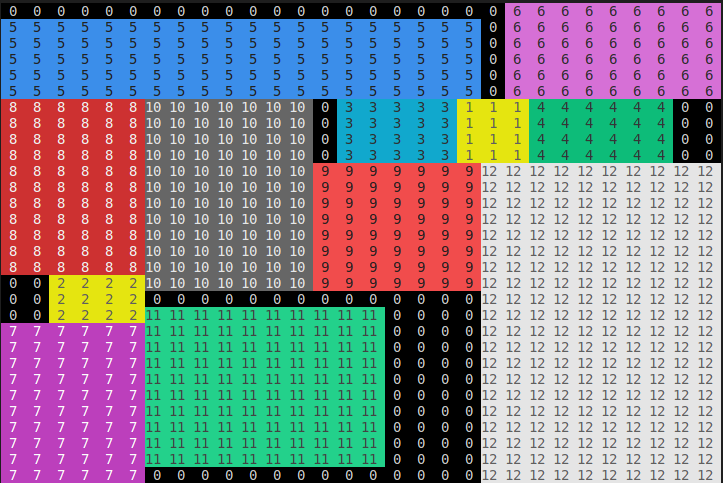
\includegraphics[width=\linewidth]{images/chipdesign_heat_16.png}

When we calculate the distance between the power components, X = $ |(19 + 1.5) - (2 + 2)| = 16 $ and Y = $  |(6 + 4) - (17+1.5)| = 8.5 $ we see that this is correct.

\subsubsection*{Heat 17}

We did this by again applying {\tt python chipdesign.py}, but this time with the heat distance value set to 17 which yields the following result within around 6 seconds.\\
sat\\

{\tt [11, 22, 4, 3]}

{\tt [7, 4, 3, 4]}

{\tt [11, 25, 4, 5]}

{\tt [11, 16, 4, 6]}

{\tt [10, 0, 20, 5]}

{\tt [2, 24, 9, 6]}

{\tt [15, 17, 10, 6]}

{\tt [0, 18, 11, 6]}

{\tt [0, 0, 7, 8]}

{\tt [15, 23, 12, 7]}

{\tt [0, 8, 10, 10]}

{\tt [10, 5, 20, 10]}\\

 Which can be visualised to show the following where components 1 and 2 are the power components:\\

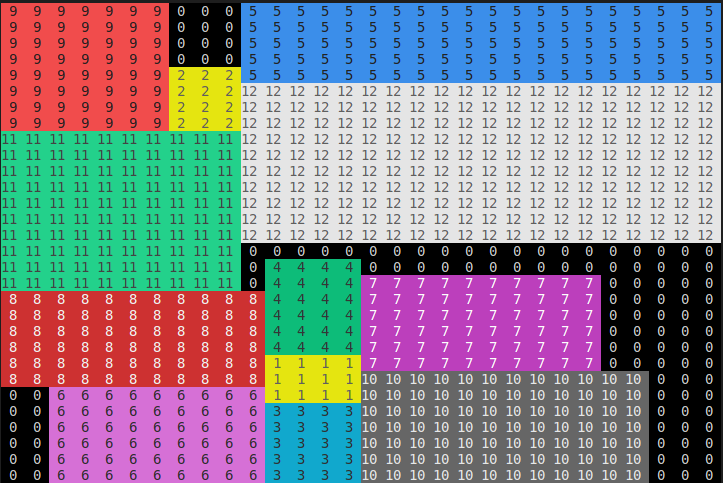
\includegraphics[width=\linewidth]{images/chipdesign_heat_17.png}

When we calculate the distance between the power components, X = $ | (11 + 2) - (7 + 1.5) | = 4.5 $ and Y = $ | (22+1.5) - (4+2) | = 17.5 $ we see that this is correct.

\subsubsection*{Heat 18}

We did this by again applying {\tt python chipdesign.py}, but this time with the heat distance value set to 17 which yields the following result within around 1 minute and 44 seconds: \\

unsat

\subsubsection*{Generalization:}

This problem can be generalized by creating a bigger chip and adding components and changing the number and size of the power components.

When defining a bigger chip with the same number of components the problem becomes easier but if we also require a lot more components to be placed and add no more power components it becomes unsat quickly since only a certain number of components can be connected to power components.

But if we also add some power components it becomes a lot harder to place all the components. Thus our solution is easily scale-able but the efficiency depends on the specific problem.

Our approach can also be used in other problems like fitting parts in 3 or 4 dimensional space by changing the structure to check for a extra dimension, for example Z in the case of 3 dimensions.

\subsection*{Problem 3: Dinner}

\subsubsection*{Problem:}
Five couples each living in a separate house want to organize a dinner. \\
Since all restaurants are closed due to some lock-down, they will do it in their own houses. \\
The dinner will consist of 5 rounds. \\
Due to the 1.5 meter restriction in every house presence of at most 5 people is allowed, by which every round has to be prepared and served in two houses simultaneously, each with the corresponding couple and three guests. \\
Every couple will serve two rounds in their house, and in between the rounds participants may move from one house to another. \\
Every two people among the 10 participants meet each other at most 4 times during these 5 rounds. Further there are four desired properties:\\

(A) Every two people among the 10 participants meet each other at least once.\\

(B) Every two people among the 10 participants meet each other at most 3 times.\\

(C) Couples never meet outside their own houses.\\

(D) For every house the six guests (three for each of the two rounds) are distinct.\\

1. Show that (A) is possible, both in combination with (C) and (D), but not with both (C) and (D).\\

2. Show that (B) is possible in combination with both (C) and (D). \\

\subsubsection*{Solution:}

We start by defining a data structure for the dinner schedule, for this we use a number of $rounds$, $houses$ and $people$. where $rounds = 5, houses=5, people=10$ \\
This leads to a $n \times m \times k$ array of Booleans where n is the number of rounds, m is the number of houses and k is the number of people. \\

Which leads to the following output, where we get 5 of these arrays, one for every round.\\
One such round:\\

{\tt [1, 1, 1, 0, 0, 1, 0, 1, 0, 0]}

{\tt [0, 0, 0, 0, 0, 0, 0, 0, 0, 0]}

{\tt [0, 0, 0, 0, 0, 0, 0, 0, 0, 0]}

{\tt [0, 0, 0, 0, 0, 0, 0, 0, 0, 0]}

{\tt [0, 0, 0, 1, 1, 0, 1, 0, 1, 1]}\\

Where every row is a house, and every column is a person. a one denotes that a person is in a house in that round.

We need to define which people are couples. we do this by providing a list that maps people to houses. if two people live in the same house they are a couple. 
We made sure that couples are next to each other in the schedule. (e.g. the first two columns are the first couple the 3rd and 4th column are the second couple etc.)  this is defined as follows: \\

\[ personToHouseIndex = \bigwedge_{p=0}^{people} \lfloor p / (\lfloor people / houses \rfloor)\rfloor \]
% person_to_house_index = [p//(NO_PEOPLE//NO_HOUSES) for p in range(NO_PEOPLE)]

This list allows us to find the house that corresponds to a given person. \\

After defining the data structure we start defining the constraints for the problem. \\
First we define some basic constraints. \\

A person is exactly in one house in each round. so we sum every column over each round where this sum must be 1. When we sum booleans we treat the booleans as integers where $false = 0$ and $true =1$ :

\[ \bigwedge_{r = 1}^{rounds} \bigwedge_{p = 1}^{people}  \sum_{h = 1}^{houses} \left( dinner\_schedule_{r,h,p} == 1 \right) \]

%# A person is exactly in one house in each round.
%one_house_at_a_time_c = [And([(sum(If(dinner_schedule[r][h][p], 1, 0) for h in range(NO_HOUSES)) == 1)
%                              for p in range(NO_PEOPLE)])for r in range(NO_ROUNDS)]

At most five people per house AND each round dinner is served in two houses. with 10 people this leads to the constraint that there are precisely 5 people per occupied house (since $10/2=5$).
Since we know that a person cannot be in multiple houses at the same time it is sufficient to say that each house has exactly 5 guests or is unoccupied:

\[ \bigwedge_{r = 1}^{rounds} \bigwedge_{h = 1}^{houses} \sum_{r=1,h=1}^{rounds,houses} \left( \left( {dinner\_schedule_{r,h}} \right) == 5 \lor \sum_{p=1}^{people} \left( {dinner\_schedule_{r,h,p}} \right) == 0 \right) \]
%# Precicely 5 people per occupied house, this implies only 2 houses are occupied.
%five_people_per_house_c = [And([Or(sumBool(dinner_schedule[r][h]) == 5, sumBool(dinner_schedule[r][h]) == 0)
%                                for h in range(NO_HOUSES)])
%                           for r in range(NO_ROUNDS)]

Each occupied house needs to have their couple in it. we check this by checking if the house is empty or if the house has it's couple in it. 
For finding the people that are in the house we could use the personToHouseIndex. but because of how the indexes align it we can use $hi*2$ and $hi*2+1$ where hi is the house index, instead. We use (h-1)*2+1 and (h-1)*2+2 since we count from 1 and not from zero:

\[ \begin{array}{c}
\bigwedge_{r = 1}^{rounds} \bigwedge_{h = 1}^{houses} ( \left({dinner\_schedule_{r,h,(h-1)*2+1} } \land {dinner\_schedule_{r,h,(h-1)*2+2}} \right) \lor \\ 
\sum_{p=1}^{people} \left( {dinner\_schedule_{r,h,p}} \right) == 0 )
\end{array} \]

%# Each occupied house needs to have their couple in it. 
%# TODO: better way to specify people based on house than h*2 and h*2+1
%each_house_its_couple_c = [And([Or(And(dinner_schedule[r][h][h*2], dinner_schedule[r][h][h*2+1]), sumBool(dinner_schedule[r][h]) == 0)
%                                for h in range(NO_HOUSES)])
%                           for r in range(NO_ROUNDS)]

Each couple is in their house exactly 2 times.
For finding the house which belongs to a person we use the personToHouseIndex, after this we can say that this person is in the corresponding house exactly 2 times. Since we do this for every person we check that every person in the couple is in their corresponding house exactly 2 times:

\[ \bigwedge_{p=1}^{people} \sum_{r=1}^{rounds} \left( {dinner\_schedule_{r,persontohouseindex_{p},p}} \right) == 2  \]

%# Each couple is in their house exactly 2 times.
%two_times_in_own_house_c = [sum(If(dinner_schedule[r][person_to_house_index[p]][p], 1, 0) for r in range(NO_ROUNDS)) == 2
%                            for p in range(NO_PEOPLE)]
% dinner_schedule[r][person_to_house_index[p]][p] for r in range(NO_ROUNDS)
Every two people among the 10 participants meet each other at most 4 times during these 5 rounds. we do this by looking at every combination of two people, then going over every round and seeing if there is at least one occurrence of both people being in the same house. we sum for each set of people how often this occurs and then just check if it is fewer or equal to 4 times:\\

 we define a lambda function:
\[Lam1_{p,p2} = \sum_{r=1}^{rounds} \left( \bigvee_{h = 1}^{houses} \left( dinner\_schedule_{r,h,p} \land dinner\_schedule_{r,h,p2} \right)  \right) <= 4\]
for every two people
\[ \bigwedge_{p=1}^{people} \bigwedge_{p2=1}^{people} \left( p <p2 \land Lam1_{p,p2}\right)  \]



%# Every two people among the 10 participants meet each other at most 4 times during these 5 rounds.
%at_most_four_c = []
%for p in range(NO_PEOPLE):
%     for p2 in range(NO_PEOPLE):
%          if(p < p2):
%               at_most_four_c.append(sumBool([Or([And(dinner_schedule[r][h][p], dinner_schedule[r][h][p2]) for h in range(NO_HOUSES)]) for r in  range(NO_ROUNDS)]) <= 4)

After defining these basic constraints we define the extra constraints A,B,C and D. \\

(A) Every two people among the 10 participants meet each other at least once. same as the "meet at most 4 times" constraints but now the number for meetings being at least 1:\\
we define a lambda function:
\[ Lam2_{p,p2} = \sum_{r=1}^{rounds} \left( \bigvee_{h = 1}^{houses} \left( dinner\_schedule_{r,h,p} \land dinner\_schedule_{r,h,p2} \right)  \right) >= 1 \]
for every two people
\[ \bigwedge_{p=1}^{people} \bigwedge_{p2=1}^{people} \left( p <p2 \land Lam2_{p,p2}\right)  \]
%# for each player: check if it shares any home and round with every other player (including itself which is by definition true.)
%a_c = []
%for p in range(NO_PEOPLE):
%     for p2 in range(NO_PEOPLE):
%          if(p < p2): a_c.append(Or([Or([And(dinner_schedule[r][h][p], dinner_schedule[r][h][p2]) for h in range(NO_HOUSES)]) for r in range(NO_ROUNDS)]))

(B) Every two people among the 10 participants meet each other at most 3 times. same as the "meet at most 4 times" constraints but now the number for meetings being at most 3:\\

we define a lambda function:
\[ Lam3_{p,p2} = \sum_{r=1}^{rounds} \left( \bigvee_{h = 1}^{houses} \left( dinner\_schedule_{r,h,p} \land dinner\_schedule_{r,h,p2} \right)  \right) <= 3 \]
for every two people
\[ \bigwedge_{p=1}^{people} \bigwedge_{p2=1}^{people} \left( p <p2 \land Lam3_{p,p2}\right)  \]

%b_c = []
%for p in range(NO_PEOPLE):
%     for p2 in range(NO_PEOPLE):
%          if(p < p2):
%               b_c.append(sumBool([Or([And(dinner_schedule[r][h][p], dinner_schedule[r][h][p2]) for h in range(NO_HOUSES)]) for r in range(NO_ROUNDS)]) <= 3)

(C) Couples never meet outside their own houses:\\
we define a lambda function:
\[ Lam4_{p1,p2,h} =\bigwedge_{r=1}^{rounds} \left( \neg \left( dinner\_schedule_{r,h,p1} \land dinner\_schedule_{r,h,p2} \right) \right)\]
for each couple and every house except theirs:
\[ \bigwedge_{c=1}^{houses} \bigwedge_{h=1}^{houses} \left( c \neq h \land Lam4_{(c-1)*2+1,(c-1)*2+2,h}\right) \]
%c_c = []
%for c in range(NO_HOUSES):
%     p1 = c*2
%     p2 = c*2+1
%     for h in range(NO_HOUSES):
%          if( h != c):
%               c_c.append(And([Not(And(dinner_schedule[r][h][p1],dinner_schedule[r][h][p2])) for r in range(NO_ROUNDS)]))

(D) For every house the six guests (three for each of the two rounds) are distinct. we check for all houses and all people not in living in that house how often they visit said house across all rounds. this must be smaller than two otherwise the same guest is not distinct:\\

\[ \bigwedge_{p=1}^{houses} \bigwedge_{p=1}^{people}  \left( persontohouseindex_{p} \neq h \land \sum_{p=1}^{rounds} \left(dinner\_schedule_{r,h,p} \right) < 2 \right)\]

%d_c = []
%for h in range(NO_HOUSES):
%     for p in range(NO_PEOPLE):
%          if(person_to_house_index[p] != h): # person not in own house
%               d_c.append(sumBool([dinner_schedule[r][h][p] for r in range(NO_ROUNDS)]) < 2)

Now that we have defined all the constraints we can show the outputs for the assignments.

\subsubsection*{1. Show that (A) is possible, both in combination with (C) and (D), but not with both (C) and (D).}

When we run the basic constraints using {\tt python dinner.py} with A and C we get the following output after 1 second:\\

sat\\

round:1\\

{\tt [0, 0, 0, 0, 0, 0, 0, 0, 0, 0]}

{\tt [0, 0, 0, 0, 0, 0, 0, 0, 0, 0]}

{\tt [0, 1, 1, 0, 1, 1, 0, 0, 0, 1]}

{\tt [1, 0, 0, 1, 0, 0, 1, 1, 1, 0]}

{\tt [0, 0, 0, 0, 0, 0, 0, 0, 0, 0]}\\

round:2\\

{\tt [1, 1, 0, 1, 1, 0, 1, 0, 0, 0]}

{\tt [0, 0, 0, 0, 0, 0, 0, 0, 0, 0]}

{\tt [0, 0, 0, 0, 0, 0, 0, 0, 0, 0]}

{\tt [0, 0, 0, 0, 0, 0, 0, 0, 0, 0]}

{\tt [0, 0, 1, 0, 0, 1, 0, 1, 1, 1]}\\

round:3\\

{\tt [0, 0, 0, 0, 0, 0, 0, 0, 0, 0]}

{\tt [0, 0, 0, 0, 0, 0, 0, 0, 0, 0]}

{\tt [0, 1, 0, 1, 1, 1, 0, 1, 0, 0]}

{\tt [0, 0, 0, 0, 0, 0, 0, 0, 0, 0]}

{\tt [1, 0, 1, 0, 0, 0, 1, 0, 1, 1]}\\

round:4\\

{\tt [0, 0, 0, 0, 0, 0, 0, 0, 0, 0]}

{\tt [1, 0, 1, 1, 1, 0, 0, 0, 0, 1]}

{\tt [0, 0, 0, 0, 0, 0, 0, 0, 0, 0]}

{\tt [0, 1, 0, 0, 0, 1, 1, 1, 1, 0]}

{\tt [0, 0, 0, 0, 0, 0, 0, 0, 0, 0]}\\

round:5\\

{\tt [1, 1, 0, 0, 0, 1, 1, 0, 0, 1]}

{\tt [0, 0, 1, 1, 1, 0, 0, 1, 1, 0]}

{\tt [0, 0, 0, 0, 0, 0, 0, 0, 0, 0]}

{\tt [0, 0, 0, 0, 0, 0, 0, 0, 0, 0]}

{\tt [0, 0, 0, 0, 0, 0, 0, 0, 0, 0]}\\

When we run the basic constraints using {\tt python dinner.py} with A and D we get the following output after around 1 second:\\

sat\\

round:1\\

{\tt [1, 1, 0, 0, 1, 1, 0, 1, 0, 0]}

{\tt [0, 0, 0, 0, 0, 0, 0, 0, 0, 0]}

{\tt [0, 0, 0, 0, 0, 0, 0, 0, 0, 0]}

{\tt [0, 0, 0, 0, 0, 0, 0, 0, 0, 0]}

{\tt [0, 0, 1, 1, 0, 0, 1, 0, 1, 1]}\\

round:2\\

{\tt [1, 1, 1, 0, 0, 0, 0, 0, 1, 1]}

{\tt [0, 0, 0, 0, 0, 0, 0, 0, 0, 0]}

{\tt [0, 0, 0, 1, 1, 1, 1, 1, 0, 0]}

{\tt [0, 0, 0, 0, 0, 0, 0, 0, 0, 0]}

{\tt [0, 0, 0, 0, 0, 0, 0, 0, 0, 0]}\\

round:3\\

{\tt [0, 0, 0, 0, 0, 0, 0, 0, 0, 0]}

{\tt [0, 0, 0, 0, 0, 0, 0, 0, 0, 0]}

{\tt [1, 0, 0, 0, 1, 1, 0, 0, 1, 1]}

{\tt [0, 1, 1, 1, 0, 0, 1, 1, 0, 0]}

{\tt [0, 0, 0, 0, 0, 0, 0, 0, 0, 0]}\\

round:4\\

{\tt [0, 0, 0, 0, 0, 0, 0, 0, 0, 0]}

{\tt [0, 1, 1, 1, 0, 1, 0, 0, 0, 1]}

{\tt [0, 0, 0, 0, 0, 0, 0, 0, 0, 0]}

{\tt [1, 0, 0, 0, 1, 0, 1, 1, 1, 0]}

{\tt [0, 0, 0, 0, 0, 0, 0, 0, 0, 0]}\\

round:5\\

{\tt [0, 0, 0, 0, 0, 0, 0, 0, 0, 0]}

{\tt [1, 0, 1, 1, 1, 0, 1, 0, 0, 0]}

{\tt [0, 0, 0, 0, 0, 0, 0, 0, 0, 0]}

{\tt [0, 0, 0, 0, 0, 0, 0, 0, 0, 0]}

{\tt [0, 1, 0, 0, 0, 1, 0, 1, 1, 1]}\\

When we run the basic constraints using {\tt python dinner.py} with A and both C and D we get the following output after around 42 seconds:\\

unsat

\subsubsection*{2. Show that (B) is possible in combination with both (C) and (D).}

When we run the basic constraints using {\tt python dinner.py} with C and D we get the following output after around 1.5 seconds :

sat\\

round:1\\

{\tt [1, 1, 0, 1, 1, 0, 0, 0, 1, 0]}

{\tt [0, 0, 0, 0, 0, 0, 0, 0, 0, 0]}

{\tt [0, 0, 0, 0, 0, 0, 0, 0, 0, 0]}

{\tt [0, 0, 1, 0, 0, 1, 1, 1, 0, 1]}

{\tt [0, 0, 0, 0, 0, 0, 0, 0, 0, 0]}\\

round:2\\

{\tt [0, 0, 0, 0, 0, 0, 0, 0, 0, 0]}

{\tt [0, 0, 0, 0, 0, 0, 0, 0, 0, 0]}

{\tt [0, 1, 1, 0, 1, 1, 0, 0, 0, 1]}

{\tt [1, 0, 0, 1, 0, 0, 1, 1, 1, 0]}

{\tt [0, 0, 0, 0, 0, 0, 0, 0, 0, 0]}\\

round:3\\

{\tt [0, 0, 0, 0, 0, 0, 0, 0, 0, 0]}

{\tt [0, 1, 1, 1, 0, 0, 0, 1, 0, 1]}

{\tt [1, 0, 0, 0, 1, 1, 1, 0, 1, 0]}

{\tt [0, 0, 0, 0, 0, 0, 0, 0, 0, 0]}

{\tt [0, 0, 0, 0, 0, 0, 0, 0, 0, 0]}\\

round:4\\

{\tt [0, 0, 0, 0, 0, 0, 0, 0, 0, 0]}

{\tt [1, 0, 1, 1, 1, 0, 1, 0, 0, 0]}

{\tt [0, 0, 0, 0, 0, 0, 0, 0, 0, 0]}

{\tt [0, 0, 0, 0, 0, 0, 0, 0, 0, 0]}

{\tt [0, 1, 0, 0, 0, 1, 0, 1, 1, 1]}\\

round:5\\

{\tt [1, 1, 1, 0, 0, 1, 0, 1, 0, 0]}

{\tt [0, 0, 0, 0, 0, 0, 0, 0, 0, 0]}

{\tt [0, 0, 0, 0, 0, 0, 0, 0, 0, 0]}

{\tt [0, 0, 0, 0, 0, 0, 0, 0, 0, 0]}

{\tt [0, 0, 0, 1, 1, 0, 1, 0, 1, 1]}\\

\subsubsection*{Generalization}

The problem can be generalised by changing the number of people,houses and rounds (these are constants in our code). Although the number of people must remain dividable across rooms of 5 people each and the number of people must consist out of couples so $NO\_PEOPLE$ must be a multiple of 10, and therefore the number of rooms must be $NO\_PEOPLE /5$. Although the constraint for the guest limit is easily changed. (This change was not needed for this exercise, agile development and all that.)


\subsection*{Problem 4: Program Safety}

\subsubsection*{Problem:}
Consider the following program:\\
{\tt a := 1; b := 1; \\
for i := 1 to 10 do \\
\indent if ? then {a := a + 2b; b := b + i} else {b := a + b; a := a + i}; \\
if b = 700 + n then crash}\\

Here ’ ?’ is an unknown test that may yield false or true in any situation. Note that the test
on crash is outside the loop, so is only tested at the end.
Establish for which values of n = 1, 2, . . . , 10 it is safe, that is, will not reach ’crash’. Show
for one of the non-safe values of n how b = 700 + n can be reached.

\subsubsection*{Solution:}
Since we want to know what the crash values are we will be negating the problem and thus searching for possible values where (b=700+n). If we find such a solution we can provide it as a non-safe value.

We use the following data structure, we have a variable for $a$ ,$b$, $i$ each round and a 0 or a 1 as a Boolean denoting what the unknown condition was to lead to this state. this Boolean for the initial 0 state is ignored.

We store these values for the different rounds in a list of size 11 (10 for the iterations of the loop and 1 for the initial state). we call this list $iter$ we also store $NO\_ROUNDS$ which is the total number of rounds, in this case 11 (10 for the loops and 1 for the in-ital state).
we use the following constraints:\\
Initial state, a b and i are all 1:
\[iter_{0,a} == 1 \land iter_{0,b} == 1 \land iter_{0,i} == 1 \]

Adjacent states have a valid transition, meaning that for each state the next state corresponds either by ${a := a + 2b; b := b + i}$ or ${b := a + b; a := a + i}$ here we make sure to also set our Boolean.
We define a lambda function:
\[ \begin{array}{c} true\_case_r  = (iter_{r +1 ,a} == iter_{r,a} + 2*iter_{r,b} \land iter_{r +1 ,b} ==  iter_{r,b}+ iter_{r,i} \\ \land iter_{r +1 ,i} == iter_{r ,i}+1 \land iter_{r +1 ,Boolean} == 1 )
\end{array} \]
We define a lambda function:
\[ \begin{array}{c} false\_case_r  = (iter_{r +1 ,a} == iter_{r,a} + iter_{r,i} \land iter_{r +1 ,b} ==  iter_{r,a} +iter_{r,b} \\ \land iter_{r +1 ,i} == iter_{r ,i}+1 \land iter_{r +1 ,Boolean } == 0 )
\end{array} \]
For all rounds 
\[ \sum_{r=0}^{NO\_ROUNDS - 1} \left(  true\_case_r \lor false\_case_r \right)\]

Final state is 700+n
\[ iter_{NO\_ROUNDS -1 ,b} == 700+n\]

Using these conditions we can let the sat solver check if for a given value of n there is a case where the last b is $700+n$ if it finds one we  know that the program can crash. if it is unsat we know that our program can never crash.
\\
We have one more condition to help speed up the program a tiny bit. We check if all the values of b are smaller or equal to $700+n$, we can do this because we see that b can never decrease. This allows us to trow out candidates quicker so that speeds it up a bit.  
\[\sum_{r=0}^{NO\_ROUNDS} \left( iter_{r,b} <= 700+n \right)\]

To get our final solution we run this solver for all n-s by executing {\tt python pragramsafety.py} and store the unsat n-s in a list and display one route when it's satisfiable. This gives us the following result after around 1.5 seconds:\\

non crashing n-s = [2, 3, 5, 7, 9]\\

To show that the program crashes for $ n = 1 $ we show the following path for the if-statements with the values for $[[a, b, i, ?]]$ where $?$ is the value for the if-statement condition. If this is 1 we set it to be true, if 0 we set it to be false.\\

round:0
{\tt[[1], [1], [1], [0]]}

round:1
{\tt[[2], [2], [2], [0]]}

round:2
{\tt[[4], [4], [3], [0]]}

round:3
{\tt[[12], [7], [4], [1]]}

round:4
{\tt[[26], [11], [5], [1]]}

round:5
{\tt[[48], [16], [6], [1]]}

round:6
{\tt[[80], [22], [7], [1]]}

round:7
{\tt[[87], [102], [8], [0]]}

round:8
{\tt[[291], [110], [9], [1]]}

round:9
{\tt[[300], [401], [10], [0]]}

round:10
{\tt[[310], [701], [11], [0]]}\\

As we can see, after round 10 the value for $b$ is 701 which is equal to $ 700 + n $ for $ n = 1$ so this path would crash.

\subsubsection*{Generalization}

This solution can be generalized for any number of rounds where we will the solver will check for 700+n for the last round. For bigger values of NO\_ROUNDS we expect the solver to get slower since it has more values to check. we also expect our optimisation condition to save more time with more rounds since the values can grow quicker. 
changing the value of n can also easily be done.
\\
The pattern we used can also be used to cover other functions than ${a := a + 2b; b := b + i}$ or ${b := a + b; a := a + i}$.
Looking at $true\_case$ and $false\_case$ we can see a simple pattern where $a := a +2b$ becomes $iter_{r +1 ,a} == iter_{r,a} + 2*iter_{r,b}$ where we say that $a$ in loop $r +1$ is defined as $a$ in loop $r$ plus two times $b$ in loop $r$. This approach also works for similar variable assignments, although more variables might be needed.

\end{document}